% Vorbereitung: Vorbereitungsaufgaben bearbeiten
% Versuchsaufbau: Verwendete Apparatur, Beschreibung Funktionsweise/Nutzen mit Skizze/Foto
\section{Durchführung}
\label{sec:durchführung}

Zunächst wird die Durchlasskurve des verwendeten Selektivverstärkers für eine Güte von $Q = 20$ untersucht, indem bei konstanter
effektiver Eingangsspannung $U_E = \qty{1}{\volt}$ unter Variation der am Sinusgenerator erzeugten Frequenz $\nu$ die
Ausgangsspannung~$U_{\! A}$ mit Verstärkungsfaktor $A_V = 1$ gemessen wird. Um in der Umgebung von $\nu_0$ eine besonders hohe
Auflösung zu erzielen, bietet sich in diesem Bereich eine entsprechend reduzierte Schrittweite beim Hochregeln von $\nu$ an.
Auf diesem Weg wird die Durchlassfrequenz $\nu_0$ des Selektivverstärkers ermittelt.

Anschließend wird eine feste Signalfrequenz $\nu = \nu_0$ eingestellt. Anstatt die Spannungsquelle direkt mit dem Filter zu verbinden,
wird mit der Sinusspannung nun die Brückenschaltung nach Abbildung \ref{fig:schaltung} gespeist. Der nachgeschaltete Linearverstärker
am Bandpass ist jetzt auf $A_V = 10$ kalibriert. Anhand Abbildung \ref{fig:schaltbild} lässt sich der Aufbau nachvollziehen, wobei der
vorgeschaltete Verstärker ausgelassen wird. Zur Verifikation der korrekten Funktion der Appartur dient ein digitales Oszilloskop, die
tatsächlichen Spannungsmessungen werden dagegen am feiner auflösenden Wechselstrom-Millivoltmeter abgelesen. 

\begin{figure}[H]
	\centering
	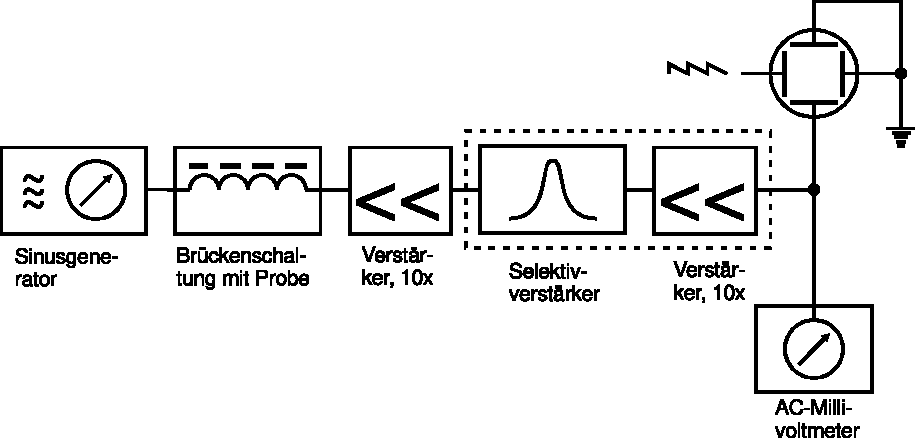
\includegraphics[width=1\linewidth]{content/grafik/schaltbild.pdf}
	\caption{Blockschaltbild der Messapparatur. Der zwischen Brücke und Filter geschaltete Verstärker
			 wird nicht verwendet \cite{paramagnet}.}
	\label{fig:schaltbild}
\end{figure}

Um die Suszeptibilität $\chi$ einer Probe bestimmen zu können, wird die freie Brücke zunächst abgeglichen. Da sich die
Spannung $\symbffrak U_\text{Br}$ nie ganz auf Null regeln lässt, wird ein Spannungsminimum eingestellt. Anschließend kann
eines der gläsernen Proberöhrchen in die dafür vorgesehene Öffnung der Messspule eingeführt werden. Nach erneutem Abgleichen
der Brückenschaltung lässt sich mittels vorheriger und neuer Stellung des Potentiometers die Widerstandsdifferenz $\increment R$
berechnen. Dieses Vorgehen wird für jede Verbindung mehrfach wiederholt. Es werden die hier pulverförmig vorliegenden Substanzen
\ce{Dy2O3}, \ce{Gd2O3} und \ce{Nd2O3} betrachtet. Zur Auswertung der Messergebnisse ist noch zu beachten, dass der
Querschnitt der Proben einer Korrektur bedarf, da sich ein Pulver in seiner Dichte von einem zusammenhängenden Kristall stark
unterscheidet. 
